% Figure 1: architecture. Build: tectonic fig1-architecture.tex, then move the PDF one level up.
\documentclass[border=1pt]{standalone}
\usepackage[T1]{fontenc}
\usepackage{libertine}
\usepackage{tikz}
\usetikzlibrary{arrows.meta, positioning}
\definecolor{eng}{HTML}{DDEFEA}
\definecolor{mod}{HTML}{E6E0F3}
\begin{document}
\hyphenpenalty=10000 \exhyphenpenalty=10000
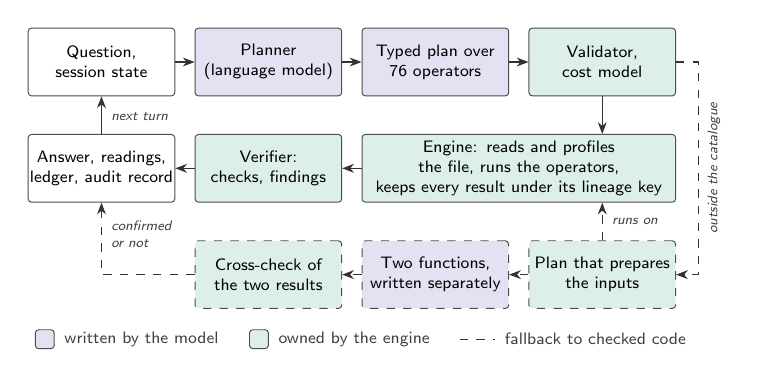
\begin{tikzpicture}[
  font=\sffamily\fontsize{6.2}{7.2}\selectfont,
  box/.style={draw=black!70, line width=0.35pt, rounded corners=1.2pt, align=center, minimum height=8.6mm, text width=18.2mm, inner sep=0.6pt},
  e/.style={box, fill=eng}, m/.style={box, fill=mod}, io/.style={box, fill=white},
  ar/.style={-{Stealth[length=1.5mm]}, line width=0.4pt, black!80},
  lab/.style={font=\sffamily\itshape\fontsize{5.4}{6.2}\selectfont, black!75}]
% row 1, left to right
\node[io] (q)  at (0,0)    {Question,\\session state};
\node[m]  (pl) at (2.12,0) {Planner\\(language model)};
\node[m]  (tp) at (4.24,0) {Typed plan over\\76 operators};
\node[e]  (va) at (6.36,0) {Validator,\\cost model};
% row 2, right to left
\node[e, text width=39.4mm] (en) at (5.3,-1.35) {Engine: reads and profiles the file, runs the operators,\\keeps every result under its lineage key};
\node[e]  (ve) at (2.12,-1.35) {Verifier:\\checks, findings};
\node[io] (an) at (0,-1.35)    {Answer, readings,\\ledger, audit record};
% row 3, fallback
\node[e, dashed]  (ip) at (6.36,-2.7) {Plan that prepares\\the inputs};
\node[m, dashed]  (cw) at (4.24,-2.7) {Two functions,\\written separately};
\node[e, dashed]  (cc) at (2.12,-2.7) {Cross-check of\\the two results};
\draw[ar] (q) -- (pl); \draw[ar] (pl) -- (tp); \draw[ar] (tp) -- (va);
\draw[ar] (va) -- (va |- en.north);
\draw[ar] (en) -- (ve); \draw[ar] (ve) -- (an);
\draw[ar] (an.north) -- node[lab, right, pos=0.45] {next turn} (q.south);
\draw[ar, dashed] (va.east) -- ++(0.28,0) |- node[lab, pos=0.25, rotate=90, anchor=north] {outside the catalogue} (ip.east);
\draw[ar, dashed] (ip) -- (cw); \draw[ar, dashed] (cw) -- (cc);
\draw[ar, dashed] (cc.west) -| node[lab, pos=0.78, right, align=left] {confirmed\\or not} (an.south);
\draw[ar, dashed] (ip.north) -- node[lab, right] {runs on} (ip |- en.south);
% legend
\node[m, minimum height=2.4mm, text width=2.4mm, inner sep=0pt] (l1) at (-0.72,-3.52) {};
\node[lab, anchor=west, font=\sffamily\fontsize{5.6}{6.4}\selectfont] at (l1.east) {written by the model};
\node[e, minimum height=2.4mm, text width=2.4mm, inner sep=0pt] (l2) at (2.0,-3.52) {};
\node[lab, anchor=west, font=\sffamily\fontsize{5.6}{6.4}\selectfont] at (l2.east) {owned by the engine};
\draw[dashed, line width=0.4pt, black!80] (4.55,-3.52) -- (5.0,-3.52);
\node[lab, anchor=west, font=\sffamily\fontsize{5.6}{6.4}\selectfont] at (5.0,-3.52) {fallback to checked code};
\end{tikzpicture}
\end{document}
